
\subsection{What You Could Get Away With}


David nodded without looking up.
``Is the synthetic hedge platform fully deployed? I want confirmation we’re delta-matched and 
neutral on spread. No physical holds — just futures, options, or swaps as needed. If we’re going 
synthetic, it better rebalance fast enough to avoid slippage, and it better not light up 
compliance across venues.''

\medskip

\begin{TechnicalSidebar}{What is a Synthetic Hedge?}

  A \textbf{synthetic hedge} is a way to mimic the protective effect of a traditional hedge without 
  holding the actual asset.  
  Instead of directly owning the asset you want to protect --- like a stock or a commodity --- you 
  construct a position using financial derivatives such as:

  \medskip

  \begin{itemize}
    \item \textbf{Futures}: contracts to buy or sell an asset at a fixed price on a future date.  

    \medskip

    \textit{Example:} You agree today to buy 1,000 barrels of oil at \$80 per barrel, delivered three months from now — even if the market price changes in the meantime.

    \medskip
  
    \item \textbf{Options}: rights (but not obligations) to buy or sell at a specific strike price before a certain date.  

    \medskip

    \textit{Example:} You pay a small premium for the right to buy a stock at \$50. If it jumps to \$70, you profit. If it drops to \$30, you let the option expire and lose only the premium.

    \medskip
  
    \item \textbf{Swaps}: agreements to exchange cash flows tied to an asset’s performance, like interest rates or stock returns.  

    \medskip

    \textit{Example:} Two companies agree to swap payments: one pays based on a fixed 3\% interest rate, the other based on whatever LIBOR is. They do this to manage different funding risks.
  \end{itemize}
  

  \medskip

  These instruments allow you to \textit{replicate} exposure, neutralize risk, or generate offsetting returns (all without 
  touching the physical asset).

  \medskip

  Synthetic hedges are faster to deploy, easier to scale across jurisdictions, and often cheaper in terms of capital 
  or regulation. But they also come with trade-offs:

  \medskip

  \begin{itemize}
    \item \textbf{Increased model risk}: due to abstraction from underlying market mechanics.  

    \medskip
    \textit{Example:} Like using a flight simulator to train for real-world flying — if the simulator has bad settings, you won’t notice real turbulence until it’s too late.
    \medskip
  
    \item \textbf{Potential for hidden leverage}: small moves in the market can lead to outsized losses because you're controlling large exposures with minimal upfront cost.  
    \medskip
    \textit{Example:} It's like putting down a 5\% deposit to control a \$1 million house — if prices drop slightly, you could still lose everything.
    \medskip
  
    \item \textbf{Sensitivity to correlation assumptions and counterparty exposure}: synthetic hedges often rely on assets moving together in predictable ways, or on counterparties honoring deals.  
    \medskip
    \textit{Example:} Imagine buying flood insurance from a neighbor who also lives on the river. If the river floods, you both lose — and your “protection” might not show up.
  \end{itemize}
  

  \medskip

  In David’s case, the synthetic hedge platform meant Arcadia could rebalance across global venues without triggering 
  the same regulatory constraints, but it also meant any misalignment could propagate faster than legacy systems 
  could catch.

\end{TechnicalSidebar}

\medskip

``Yep. EU regulation’s lighter on delta thresholds. We have more elasticity on notional wraps,'' she said, 
scrolling through the live monitor.


\medskip

\begin{TechnicalSidebar}{What Are Delta Thresholds?}

  In trading, \textbf{delta} measures how much the value of a position changes in response to a change in the price 
  of the underlying asset.  
  A delta of 1.0 means a \$1 move in the asset causes a \$1 move in the position. A delta of 0.5 means only a \$0.50 
  move, and so on.

  \medskip

  \textbf{Delta thresholds} are regulatory or internal risk limits that restrict how much directional exposure a 
  portfolio or synthetic instrument can carry.  
  These thresholds are especially important for complex or leveraged positions, such as:

  \medskip

  \begin{itemize}
    \item \textbf{Derivatives with embedded leverage}: financial contracts that let you control a large position with a small upfront cost.  

    \medskip

    \textit{Example:} Like renting a Ferrari for the price of a scooter — you get speed and power, but if you crash, the bill is still full-sized.

    \medskip
  
    \item \textbf{Synthetic swaps or basket trades}: complex financial instruments that mimic the behavior of multiple underlying assets, often without holding any of them directly.  

    \medskip

    \textit{Example:} Like betting on the combined scores of five sports teams without watching any of the games — you win or lose based on an index you don’t actually control.

    \medskip
  
    \item \textbf{Algorithmically generated hedges}: risk protection strategies automatically built and adjusted by computer models, often in real time.  

    \medskip

    \textit{Example:} Like a self-driving car that constantly changes lanes to avoid traffic — fast and responsive, but if the sensors are off, it might drive straight into a wall.
  \end{itemize}
  

  \medskip

  Tighter delta thresholds mean tighter control — trades must stay close to neutral or hedged exposure.  
  Looser thresholds allow greater directional bets, larger notional swings, and more elasticity in how positions 
  are wrapped and deployed.

  \medskip

  In this case, EU regulation being “lighter on delta thresholds” means the model can take on more delta — more 
  market sensitivity —  
  without triggering a compliance block. It creates flexibility, but also introduces risk: the system can swing 
  wider before hitting a stop.

\end{TechnicalSidebar}

\medskip

``We’ve got no physical exposure on the books. All synthetic. Mix of short-dated futures for the front 
leg, plus some laddered calls in London and Frankfurt. The swaps desk’s holding neutral — delta-matched 
within 10 basis points. We set the auto-rebalance to trigger if correlation assumptions break outside 
tolerance.''

She looked up. ``No compliance flags so far. Liquidity bands holding. And if it moves too fast, we’ve 
got unwind logic pre-wired by venue.''
A pause. ``It’s quiet now, but the system’s listening.''

The words that landed were clean, confident, and factual.
But in his mind, they echoed with the ghost of a whiteboard marker squeaking on glass.

He was back in Luxembourg.

Not for the scenery. Not for the tax code — though that helped.

The meeting had to be there because that’s where the carve-out lived.
A bespoke entity, ring-fenced for jurisdictional flexibility and structured just thinly enough to avoid tripping oversight triggers in London or New York.

Luxembourg offered what the others couldn't:
\textit{neutrality without scrutiny.}
A sandbox for structured exposure.
A place where reporting thresholds were softer, risk categorization more pliable, and synthetic instruments could be tested just outside the perimeter of consolidated supervision.

The lawyers had called it “geo-optimization.”
The structurers called it “the buffer.”
David called it what it was: plausible deniability.

They didn’t bring full teams. Just enough people to call it a workshop.
Enough ambiguity to avoid board minutes, but enough technical clarity to push the boundary of the architecture.

They filled the whiteboard in layers — venue behavior, stress scenarios, cross-currency overlays.
But underneath it all was the same unspoken question:

What can we get away with… if the delta doesn’t spike?

That was the real reason they flew to Luxembourg.
Not for strategy.
But for insulation.
For a place to ask the wrong questions — and not be told no.

\medskip

\begin{HistoricalSidebar}{Why Luxembourg? A Soft-Law Capital for Hard-Money Games}

    Luxembourg may be smaller than Rhode Island, but in structured finance, size isn’t the metric that matters.

    \medskip
    
    What matters is architecture — legal, fiscal, and regulatory.
    
    \medskip
    
    Since the 1990s, Luxembourg has become a global hub for structured investment vehicles (SIVs), special purpose entities (SPEs), and cross-border funds. Not because it’s secretive in the Swiss sense, but because it offers a uniquely accommodating legal environment:

    \medskip
    
    \begin{itemize}
    \item \textbf{Flexible entity structures:} From the Société d’Investissement à Capital Variable (SICAV) to the newer RAIF (Reserved Alternative Investment Fund), Luxembourg lets you match your entity structure to your risk appetite.
    
    \item \textbf{Light-touch regulation:} Funds can operate under “passporting” rules via EU directives (like UCITS or AIFMD), but in practice, certain structures avoid full supervisory friction — especially if they’re not publicly distributed.
    
    \item \textbf{Tax efficiency without scandal:} Luxembourg isn’t a blacklisted tax haven. It’s OECD-compliant, but its double-tax treaties, thin-cap rules, and tolerance for hybrid instruments make it a favorite for optimizing exposure without lighting compliance alarms.
    \end{itemize}
    
    \medskip
    
    So why fly there?

    \medskip
    
    Because while the \textbf{war room is in New York}, the risk architecture is often offshore — not just in geography, but in logic.
    
    \medskip
    
    \begin{itemize}
    \item New York is where the trades happen.
    \item Luxembourg is where the liabilities sleep.
    \end{itemize}
    
    That’s why deal teams meet there.

    \medskip
    
    Not to decide strategy — but to shape the vessel that will carry it.

    \medskip
    
    In Luxembourg, conversations aren’t recorded. Term sheets are reviewed in person. And “structure” becomes a verb.
    
    \medskip
    
    It’s not about hiding. It’s about anchoring the legal fiction in the right jurisdiction.

    \medskip
    
    Because once the entity is domiciled, the map — and the rules — change.
    
\end{HistoricalSidebar}

\medskip

Not the conference room — the smaller one. The off-calendar prep call before the vendor roadshow.
Where the conversation hadn’t been about compliance. It had been about \textit{what you could get 
away with, if the delta didn’t spike}.

\textit{“We wrap it tight — low delta, small notional, but levered exposure.”}
That had been Sofia from structuring. Calm, like she was describing the weather.

\begin{TechnicalSidebar}{The Structuring Desk — Architects of Financial Engineering}

    In modern finance, the \textbf{structuring team} sits at the intersection of product design, 
    legal arbitrage, and quantitative engineering.
    
    They don’t pitch.  
    They don’t execute.  
    They build.
    
    \bigskip
    
    \textbf{What do they structure?}  
    Custom financial products — often bespoke derivatives, wrapped securities, or hybrid instruments 
    that don’t fit into clean categories.
    
    \begin{itemize}
      \item \textbf{Total Return Swaps (TRS)}
      \item \textbf{Synthetic ETFs}
      \item \textbf{Credit-Linked Notes (CLNs)}
      \item \textbf{Volatility-controlled wrappers}
    \end{itemize}
    
    \bigskip
    
    \textbf{Why does it matter?}
    
    Because structurers don’t just ask,  
    \begin{quote}
      \textit{“What’s the exposure?”}  
    \end{quote}
    They ask,  
    \begin{quote}
      While delivering the same risk,
      how can we wrap this exposure to satisfy compliance, balance sheet constraints, and 
      marketing optics?
    \end{quote}
    
    \bigskip
    
    \textbf{Three core mandates:}
    
    \begin{itemize}
      \item \textbf{Regulatory Awareness:}  
      Know the edge of the rulebook — and how to stay just inside it.
    
      \item \textbf{Risk Translation:}  
      Convert complex exposures into more palatable formats (e.g., lower delta, lower notional, higher leverage).
    
      \item \textbf{Sales Enablement:}  
      Make the exotic feel ordinary.  
      If a trader sells volatility, the structurer wraps it in something the client can understand — or legally hold.
    \end{itemize}
    
    \bigskip
    
    \textbf{A Structurer’s Motto (Unofficial):}  
    \begin{quote}
      “If you can’t move the risk, move the wrapper.”
    \end{quote}
    
    Which is why in prep calls and quiet rooms, the question isn’t “Is it compliant?”  
    It’s:  
    \begin{quote}
      \textit{“Can we show the optics without the spikes?”}
    \end{quote}
    
    Because in structured products, what’s \textbf{visible} often matters more than what’s \textbf{real}.
    

\end{TechnicalSidebar}

\medskip

Sophia let the words settle, then glanced around the room — not condescending, just aware that not 
everyone operated at her altitude.

“Just to level-set,” she said. “There are three ways to chase exposure. You can go high delta, high 
notional — that’s brute force. It tracks the underlying precisely, but it also triggers every compliance 
alert from here to Delaware.”

A few nods.

“Or you can go high notional, low delta — like macro overlays. Looks clean on paper but gets messy when 
rates shift or basis moves.”

She tapped the term sheet lightly.

“We choose the third lane: low delta, small notional, high leverage. That way the instruments don’t shout 
position. They whisper. You get the same directional profile without tripping any wires.”

\medskip


\begin{table}[H]
\centering
\caption{Comparison of Exposure Strategies}
\begin{tabularx}{\textwidth}{|X|X|X|X|}
\hline
\textbf{Strategy} & \textbf{Delta / Notional} & \textbf{Use Case} & \textbf{Trade-Offs} \\
\hline
\textbf{Brute Force} & High delta, high notional & Precise tracking of underlying asset & Full transparency, triggers compliance alerts \\
\hline
\textbf{Macro Overlay} & Low delta, high notional & Broad hedging or directional bias & Clean optics, but unstable if rates or basis shift \\
\hline
\textbf{Disclosure-Efficient} & Low delta, low notional, high leverage & Quiet directional exposure & Stays under radar, but needs constant monitoring and rebalancing \\
\hline
\end{tabularx}
\end{table}



\medskip








Someone asked — carefully, not confrontational —
“Don’t we need swap disclosure?”

It was Nathan — the junior from London, fresh off his Series 7 and still reading footnotes like they 
were commandments.

\medskip

\begin{TechnicalSidebar}{Swap Disclosure: What Must Be Reported, and When}

    Under U.S. financial regulation, \textbf{swaps} --- particularly \textbf{total return swaps (TRS)} and 
    other derivatives --- are subject to reporting requirements depending on their structure, counterparties, 
    and systemic risk potential.
    
    \medskip
    
    Key regulatory frameworks include:
    
    \medskip
    
    \begin{itemize}
      \item \textbf{Dodd-Frank Act} (2010): Requires many swaps to be reported to \textbf{Swap Data Repositories (SDRs)}.
      \item \textbf{SEC Rules 13D and 13G}: May trigger public disclosure if the swap gives beneficial ownership 
      or control over more than 5\% of a company's voting shares.
      \item \textbf{CFTC Reporting}: Mandates real-time and post-trade reporting of certain swap details (counterparty, 
      notional amount, pricing).
    \end{itemize}
    
    \medskip
    
    \textbf{However:} Disclosure may not be required if:

    
    \medskip
    
    \begin{itemize}
      \item The swap does not confer voting rights or control.
      \item The notional exposure remains below regulatory thresholds.
      \item The transaction is conducted through exempt counterparties or offshore entities.
    \end{itemize}
    
    \medskip
    
    \textbf{Layman Example:}  
    Imagine a hedge fund wants exposure to 4.9\% of a company’s stock without triggering public ownership filings.  
    Instead of buying shares directly, they enter a \textbf{total return swap} with a bank, which holds the shares 
    on its balance sheet.  
    The fund receives profits (or losses) as if it owned the shares — but since it technically doesn’t, no 13D 
    filing is required.  
    To the public, the fund appears uninvolved.  
    To the market, it's invisible.  
    But economically, it holds the same stake.
    
\end{TechnicalSidebar}

\medskip

Sofia didn’t flinch. She was smoothing her cuff, not even looking up from the term sheet.

“Not if the exposure stays within bounds,” she said calmly.

Nathan blinked. “But—sorry—aren’t swaps, like, reportable under Dodd-Frank? If we’re using them to 
replicate a position, isn’t that... material?”

She finally looked at him. Not annoyed. Not amused. Just… steady.

“Material to whom?” she asked. “The client? Compliance? The SEC?”

He hesitated. “Well... all of them?”

A few quiet chuckles around the table.

Sofia leaned back, folding her hands loosely.

“Okay, Nathan,” she said, “think of it like this. Let’s say you want to carry water across the border. 
Big jugs of water. But the customs limit says one liter per person.”

He nodded, still a little lost.

“So,” she continued, “you don’t bring one giant jug. You bring four friends. Everyone carries a liter. 
All within the limit. No flags raised.”

“That’s legal?”

She smiled faintly. “It’s within regulation. That’s the game.”

Nathan frowned. “But it’s still four liters of water.”

“Right,” she said. “But not in one container. Same with swaps. One big exposure triggers scrutiny. 
But split it — limit the notional, keep the delta low, rebalance frequently — and it stays under the 
radar.”

He leaned forward, trying to catch up. “So... it’s like smuggling, but politely?”

Sofia tilted her head. “It’s disclosure-efficient structuring.”

Someone else chimed in. “It’s not about hiding. It’s about not shouting.”

“And if the risk spikes?” Nathan asked.

“That’s what limits are for,” she said. “We pre-wire the unwind. We use triggers. If the exposure 
steps out of bounds, we step out of the position.”

He sat back, still chewing on the metaphor.

“You’re thinking in ethics,” she said gently. “We think in thresholds.”

And just like that, the meeting moved on.

\medskip

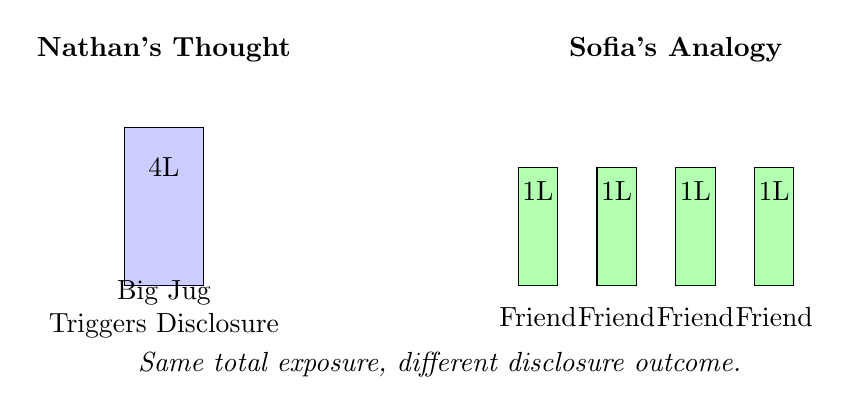
\begin{tikzpicture}

    % Title labels
    \node[align=center, font=\bfseries] at (1.5, 4) {Nathan's Thought};
    \node[align=center, font=\bfseries] at (8, 4) {Sofia's Analogy};
    
    % Nathan's Big Jug
    \draw[fill=blue!20, draw=black] (1,1) rectangle ++(1,2);
    \node at (1.5,2.5) {4L};
    \node[align=center] at (1.5,0.7) {Big Jug\\Triggers Disclosure};
    
    % Sofia's Small Jugs
    \foreach \i in {0,1,2,3} {
      \draw[fill=green!30, draw=black] (6+\i*1,1) rectangle ++(0.5,1.5);
      \node at (6.25+\i*1,2.2) {1L};
      \node[align=center] at (6.25+\i*1,0.6) {Friend};
    }
    
    % Caption
    \node[align=center, font=\itshape] at (5,0) 
      {Same total exposure, different disclosure outcome.};
    
\end{tikzpicture}

\medskip

\begin{HistoricalSidebar}{Dodd-Frank and the Illusion of Transparency}

    The \textbf{Dodd–Frank Wall Street Reform and Consumer Protection Act} was signed into law in 2010, 
    a sweeping response to the 2008 financial crisis. It promised accountability, oversight, and above 
    all: transparency.
    
    \medskip
    
    At its core, Dodd-Frank aimed to shine a light on the shadowy corners of finance — especially on 
    derivatives like \textbf{total return swaps}, \textbf{credit default swaps}, and other off-balance-sheet 
    magic tricks that helped implode global markets.
    
    \medskip
    
    Among its tools:

    \medskip
    
    
    \begin{itemize}
      \item \textbf{Title VII} regulated derivatives trading through central clearing and real-time reporting.
      \item \textbf{Section 13} (a.k.a. the Volcker Rule) restricted proprietary trading by banks.
      \item \textbf{Office of Financial Research (OFR)} was created to monitor systemic risk.
    \end{itemize}
    
    \medskip
    
    But as always, reform met reality.

    \medskip
   
    \begin{itemize}
        \item \textbf{Reporting thresholds were raised.}
        \item \textbf{Loopholes were rebranded as exemptions.}
        \item \textbf{Enforcement got outsourced to interpretation.}
    \end{itemize}
    
    \medskip
    
    Firms didn’t stop structuring risk.

    \medskip
    
    They just started calling it something else.
    
    \medskip
    
    By 2020, private funds had perfected the art of \textbf{economic exposure without legal ownership}. Swaps 
    became mirrors that let investors “replicate” positions without triggering disclosures meant for 
    actual shareholders.
    
    \medskip
    
    So yes, Dodd-Frank technically requires swap disclosure.

    \medskip
    
    But as Sofia understood — and Nathan was still learning — \textit{technicality is a poor substitute 
    for enforcement}.
    
\end{HistoricalSidebar}

\medskip

David had stared at the model on screen.
An options tree with synthetic deltas shaded like heat zones.

It was beautiful, in a terrifying way — a branching lattice of possibilities, each node a 
conditional future priced in microseconds.
The paler regions were low-risk: hedged, capped, buffered by structure.
But the deeper reds — they glowed like warning flares.

Those were the trades with teeth.
The ones with leverage baked in.
The ones that looked stable at the surface but spiked in exposure when the wind changed by 
half a basis point.

Each shade wasn’t just a number.
It was a bet.
A bet on volatility. On liquidity. On the assumption that nothing — not rates, not sentiment, 
not regulators — would move too fast.

He zoomed in. A single node, labeled 0.82 delta, flared crimson.
That one alone could tip the balance sheet if liquidity dried up.

The tree didn’t lie.
It just didn’t warn you when it was hungry.

David exhaled.
This wasn’t risk modeling anymore.
This was choreography — a delicate, probabilistic ballet performed on a stage where the floor might collapse without notice.

\medskip


\begin{figure}[H]
    \centering
    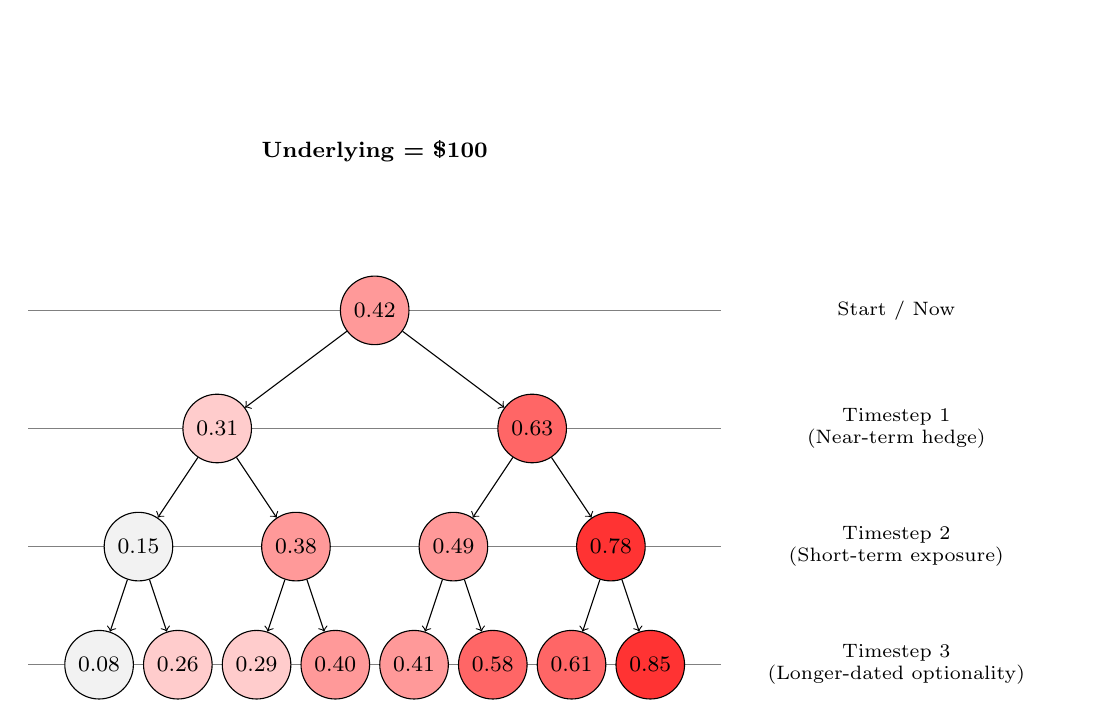
\begin{tikzpicture}[
        level distance=1.5cm,
        level 1/.style={sibling distance=4cm},
        level 2/.style={sibling distance=2cm},
        level 3/.style={sibling distance=1cm},
        every node/.style={circle, draw, minimum size=0.8cm, font=\footnotesize, text=black},
        edge from parent/.style={draw, ->}
      ]
  
      % Color definitions for synthetic deltas
      \tikzset{
        hot0/.style={fill=black!5},
        hot1/.style={fill=red!20},
        hot2/.style={fill=red!40},
        hot3/.style={fill=red!60},
        hot4/.style={fill=red!80}
      }

      \draw[solid, gray] (-4.4,0) -- (4.4,0) 
        node[right, font=\scriptsize, draw=none, fill=none, shape=rectangle] 
        {\parbox{4.2cm}{\centering Start / Now}};
      \draw[solid, gray] (-4.4,-1.5) -- (4.4,-1.5) 
        node[right, font=\scriptsize, draw=none, fill=none, shape=rectangle] 
        {\parbox{4.2cm}{\centering Timestep 1\\(Near-term hedge)}};
      \draw[solid, gray] (-4.4,-3) -- (4.4,-3) 
        node[right, font=\scriptsize, draw=none, fill=none, shape=rectangle] 
        {\parbox{4.2cm}{\centering Timestep 2\\ (Short-term exposure)}};
      \draw[solid, gray] (-4.4,-4.5) -- (4.4,-4.5) 
        node[right, font=\scriptsize, draw=none, fill=none, shape=rectangle] 
        {\parbox{4.2cm}{\centering Timestep 3\\ (Longer-dated optionality)}};
  
      % Tree definition with synthetic delta intensity
      \node[hot2, label=above:{\textbf{Underlying = \$100}}] {0.42}
        child {node[hot1] {0.31}
          child {node[hot0] {0.15}
            child {node[hot0] {0.08}}
            child {node[hot1] {0.26}}
          }
          child {node[hot2] {0.38}
            child {node[hot1] {0.29}}
            child {node[hot2] {0.40}}
          }
        }
        child {node[hot3] {0.63}
          child {node[hot2] {0.49}
            child {node[hot2] {0.41}}
            child {node[hot3] {0.58}}
          }
          child {node[hot4] {0.78}
            child {node[hot3] {0.61}}
            child {node[hot4] {0.85}}
          }
        };
  
    \end{tikzpicture}
  
    \vspace{1em}
  
    \begin{tabular}{|c|c|}
      \hline
      \textbf{Delta Range} & \textbf{Visual Cue / Interpretation} \\
      \hline
      $\delta < 0.2$ & \cellcolor{black!5} Lightest — Minimal directional sensitivity \\
      $0.2 \leq \delta < 0.4$ & \cellcolor{red!20} Low-moderate exposure \\
      $0.4 \leq \delta < 0.6$ & \cellcolor{red!40} Balanced option exposure \\
      $0.6 \leq \delta < 0.8$ & \cellcolor{red!60} High directional correlation \\
      $\delta \geq 0.8$ & \cellcolor{red!80} Near-linear tracking with underlying asset \\
      \hline
    \end{tabular}
  
    \caption{Options Tree Visualization with Time-Labeled Rows and Delta Intensity Heatmap}
\end{figure}



\medskip


He had asked:
“What's the elasticity look like under stress?”

Sofia:
\textit{“Better than real. Because we’re modeling control, not cash.”}

Someone else:
\textit{“If real hedges cost too much, synthetics give you a pass.”}

David remembered the way that felt. Not wrong — just fast.
A feeling that the trade wasn't being made. It was being described into existence.

He had said yes. Eventually.
Because when the desk asked for exposure without visibility,
synthetics were the answer that didn’t have to be explained in the audit notes —
only in the footnotes.

\medskip

Back in London now, he stared out over the skyline,
remembering how they’d phrased it:
\textit{“EU reg lets us flex the wrap.”}

Flex. Not “hedge.” Not “protect.”
Just... flex.

And he wondered, not for the first time,
if elasticity was just another word for a loophole
you haven't been caught using yet.


“And the latency?”

“Thirty-seven milliseconds desk to desk. Aurora’s already ported the model footprint to the London grid. 
Real-time sync across venues.”

\medskip

\begin{TechnicalSidebar}{Why Latency Matters in Trading}

  \textbf{Latency} refers to the delay between the moment a trading signal is generated and when it 
  is executed on an exchange.  
  In high-frequency and cross-venue trading, even a few milliseconds can mean the difference 
  between arbitrage and loss.

  \medskip

  \textbf{Thirty-seven milliseconds desk to desk} might sound fast, but in trading terms, it’s an eternity 
  compared to sub-millisecond co-located systems.  

  \medskip

  That latency includes:

  \begin{itemize}
    \item Signal generation and transmission
    \item Routing across network hops (e.g., New York to London)
    \item Exchange confirmation and roundtrip acknowledgment
  \end{itemize}

  \medskip

  \textbf{Porting the model to the London grid} means Aurora reduced some of that latency by 
  shifting compute closer to the venue.  
  Real-time synchronization across venues ensures consistency in state, but only if latency 
  is stable and predictable.

  \medskip

  In this case, 37ms is a performance ceiling.  
  It defines how reactive the system can be under stress, and how quickly risk can be 
  neutralized when the market turns.

\end{TechnicalSidebar}

\medskip

David leaned back, eyes scanning the floor. It looked calm.
It always did right before.



